\documentclass[12pt, a5paper, parskip=half-]{scrartcl}

% Adjust spacing before and after section headings
\RedeclareSectionCommand[
  runin=false,
  beforeskip=\baselineskip,
  afterskip=-0.25\baselineskip
]{section}

\RedeclareSectionCommand[
  runin=false,
  beforeskip=0.5\baselineskip,
  afterskip=-0.25\baselineskip
]{subsection}

\RedeclareSectionCommand[
  runin=false,
  beforeskip=0.5\baselineskip,
  afterskip=-0.25\baselineskip
]{subsubsection}

%\usepackage[pass]{geometry}
\usepackage{fontspec} % Use system fonts.  Not compatible with pdflatex. Use XeLaTeX instead!
\usepackage{cinzel}
 \newfontfamily\displayfont{Cinzel}
\setkomafont{section}{\large\cinzel\bfseries}
\setkomafont{subsection}{\cinzel\bfseries}
\setkomafont{subsubsection}{\cinzel\bfseries}


\usepackage{enumitem} % Adjust formatting of description environment items

\usepackage{multicol} % Format list of playtesters in two columns

%\usepackage[pages=some, color=black]{background}
%\backgroundsetup{
%firstpage=true,
%color=black,
%opacity=1,
%angle=0,
%scale=1,
%contents = {%
%    
\includegraphics[width=\paperwidth,height=\paperheight]{Images/booklet_cover_background.jpg}
%  }%
%}

%dice mini-diagrams
\usepackage{tikz}
\usetikzlibrary{arrows.meta}
\usetikzlibrary{shapes}
\usetikzlibrary{calc}
\usetikzlibrary{decorations.pathmorphing}

\tikzset{die1/.pic={
    	\node[draw, very thick,minimum size=1em, rounded corners=1mm] {};
    	\node[draw, fill=black, circle, inner sep=0.65pt] {};
	}
}

\tikzset{die2/.pic={
    	\node[draw, very thick,minimum size=1em, rounded corners=1mm] {};
    	\node[draw, fill=black, circle, inner sep=0.65pt] at (0.1, 0.1) {};
    	\node[draw, fill=black, circle, inner sep=0.65pt] at (-0.1,  -0.1) {};
	}
}

\tikzset{die3/.pic={
    	\node[draw, very thick,minimum size=1em, rounded corners=1mm] {};
    	\node[draw, fill=black, circle, inner sep=0.65pt] {};
    	\node[draw, fill=black, circle, inner sep=0.65pt] at (0.1, 0.1) {};
    	\node[draw, fill=black, circle, inner sep=0.65pt] at (-0.1,  -0.1) {};
	}
}

\tikzset{die4/.pic={
    	\node[draw, very thick,minimum size=1em, rounded corners=1mm] {};
    	\node[draw, fill=black, circle, inner sep=0.65pt] at (0.1, 0.1) {};
    	\node[draw, fill=black, circle, inner sep=0.65pt] at (0.1, -0.1) {};
    	\node[draw, fill=black, circle, inner sep=0.65pt] at (-0.1, 0.1) {};
    	\node[draw, fill=black, circle, inner sep=0.65pt] at (-0.1,  -0.1) {};
	}
}

\tikzset{die5/.pic={
    	\node[draw, very thick,minimum size=1em, rounded corners=1mm] {};
    	\node[draw, fill=black, circle, inner sep=0.65pt] {};
    	\node[draw, fill=black, circle, inner sep=0.65pt] at (0.1, 0.1) {};
    	\node[draw, fill=black, circle, inner sep=0.65pt] at (-0.1,  -0.1) {};
    	\node[draw, fill=black, circle, inner sep=0.65pt] at (0.1, -0.1) {};
    	\node[draw, fill=black, circle, inner sep=0.65pt] at (-0.1,  0.1) {};

	}
}

\tikzset{die6/.pic={
    	\node[draw, very thick,minimum size=1em, rounded corners=1mm] {};
     \node[draw, fill=black, circle, inner sep=0.65pt] at (0.1, 0.1) {};
    	\node[draw, fill=black, circle, inner sep=0.65pt] at (-0.1,  -0.1) {};
    	\node[draw, fill=black, circle, inner sep=0.65pt] at (0.1, -0.1) {};
    	\node[draw, fill=black, circle, inner sep=0.65pt] at (-0.1,  0.1) {};
    	\node[draw, fill=black, circle, inner sep=0.65pt] at (-0.1,  0) {};
    	\node[draw, fill=black, circle, inner sep=0.65pt] at (0.1, 0) {};

	}
}

%fancy page numbers
\renewcommand{\pagemark}
{

\begin{tikzpicture}[scale=0.2]
%\node[draw, star, star points = 8, star point ratio = 0.5, rounded corners=0.8mm, minimum size=0.8cm, thick, rotate=35] (a) at (0,0) {};
\node[draw, star, star points = 9, star point ratio = 0.5, rounded corners=1.25mm, minimum size=3.0cm, semithick, rotate=27.5, transform shape] (a) at (0,0) {};
	\foreach \i in {0,1,2,3,4,5,6,7,8}
		\node[draw, circle, semithick, transform shape, minimum size=0.45cm] (a\i) at (40*\i + 1:2.75cm) {};

\node (b) at (0,0) {\arabic{page}};
%\foreach \i in {0,1,2,3,4,5,6,7}
%	\node[draw,circle,inner sep=0.5mm, thick] (\i) at (45*\i - 12.5:0.7) {};
\node at (0,6.5) {};
\end{tikzpicture}
}

\begin{document}
%=========================================
\begin{titlepage}
		\enlargethispage{5\baselineskip}

         \setmainfont{Cinzel Decorative}
	    \centering{
			{\fontsize{60}{72}\selectfont
			{\textcolor{black}{pROpHecY}}}
		}
%         \setmainfont{Muli}
%	    \centering{
%			{\fontsize{60}{72}\selectfont
%			{\textcolor{black}{PROPHECY}}}
%		}


		\setmainfont{URWClassico}
		\vspace{10mm}
%		\centering{\Large{{\textcolor{lightgray}
%{A tabletop roleplaying game\\ \smallskip about fate and destiny}}}}
		\centering{\Large{{\textcolor{black}
{A tabletop roleplaying game\\ \smallskip about fate and destiny}}}}

\vfill

\includegraphics[scale=3.85]{Images/comet_diagram.pdf}

		\vfill
		
%		\raggedright{\Large{{\textcolor{lightgray}{Michael Purcell \hfill November 2021}}}}
		\raggedright{\Large{{\textcolor{black}{Michael Purcell \hfill November 2021}}}}

\end{titlepage}


%=========================================

\setmainfont{URWClassico}
%\setmainfont{Muli}
\normalsize
\raggedright
\section*{Introduction}
Prophecy is a tabletop roleplaying game about fate and destiny. During the game, the players receive a prophecy that describes an impending catastrophe for some fictional world. They create characters who inhabit that fictional world, write an outline that describes how their characters will try to deal with the catastrophe, and tell the story of their characters' adventures.

Throughout these rules, a variety of common words are used as technical terms to describe how the game is played. These terms will be Capitalised when they appear in the text and \emph{Italicised} when they are first introduced.
%Occasionally, the rules described in one section will refer to rules described in another section.
%When this happens, the reference will consist of a hyperlink to the target section.
%The link text will be the title of the target section.

\section*{Materials}
To play the game, the players will need a few materials that they will use to take notes and generate random numbers. They will need:
\begin{description}[leftmargin=0pt]
	\item[Index Cards] Approximately fifty index cards should placed within easy reach of all players. 
	\item[Sticky Notes] Approximately one hundred sticky notes should placed within easy reach of all players.
	\item[Butcher Paper]	 One large sheet of butcher paper should be placed in the middle of the play area.  This is the \emph{Story Board}. A whiteboard can be used instead if desired.
	\item[Markers] Each player should have a marker that they can use to write on the index cards, sticky notes, and Story Board.
	\item[Dice] Approximately twelve six-sided dice should be placed within easy reach of all players. 
\end{description}

\newpage

\section*{Mechanics}    
\emph{Mechanics} are the systems that govern how players interact with the game.
They provide a way for players to describe a fictional world by populating it with Objects and Aspects, compose a story set in that world by describing Scenes, and determine how that story plays out by making Checks.

\subsection*{Objects and Aspects}
An \emph{Object} is a person, place, or thing that appears in the story.
An \emph{Aspect} is a word or short phrase that describes something noteworthy about an Object.
Each Aspect is \emph{Attached} to a single Object.

The players should use an index card to represent each Object and a sticky note to represent each Aspect.  If an Aspect is Attached to an Object, then the players should stick the sticky note representing that Aspect to the index card representing that Object.

\subsubsection*{Characters}
A \emph{Character} is a person who appears in the story and whose actions will be controlled by a single player throughout the game.  An Aspect that is Attached to a Character is a \emph{Character Aspect}.
An Aspect that is Attached to any Object that is not a Character is an \emph{Environment Aspect}.

\subsubsection*{Matching Aspects}
A pair of \emph{Matching Aspects} is a set of two Aspects, one Character Aspect and one Environment Aspect, that together allow the Characters to manipulate a Scene to their advantage.

\newpage

\subsection*{Scenes}
A \emph{Scene} is a part of the story that describes the events that happen at a single time and place.
Every Scene has the following components:
\begin{description}[leftmargin=0pt]
  \item[\emph{Setting}]
  The time and place at which the Scene occurs. The Setting includes the Objects and Aspects that appear in the Scene.
  \item[\emph{Objective}]
    A narrative description of what the Characters are trying to accomplish during the Scene.
  \item[\emph{Difficulty Rating}]
    A number that describes how difficult it is for the Characters to accomplish the Scene's Objective.
  \item[\emph{Outcome}]
    A description of whether the Characters accomplish the Scene's Objective. If so, then the Outcome is a \emph{Success} and the Scene is resolved successfully. Otherwise, the Outcome is a \emph{Failure} and the Scene is resolved unsuccessfully.
  \item[\emph{Precursors}]
    Other Scenes which, if resolved successfully, make it easier for the Characters to accomplish the Scene's Objective. A Scene is the \emph{Parent} of all of its Precursors.
\end{description}


\newpage

\subsubsection*{Sketching Scenes}
The players \emph{Sketch} Scenes when they Write an Outline describing the story that they will tell about the Characters. To Sketch a Scene the players will establish the Setting, define the Objective, and assign the Difficulty Rating for the Scene.

The players should use an oval drawn on the Story Board to represent each Scene. The oval that represents a Scene should be labelled with that Scene's Objective and Difficulty Rating.  The players should draw lines connecting the oval that represents each Scene to the ovals that represent its Precursors.


\subsubsection*{Performing Scenes}
The players \emph{Perform} Scenes when they Tell the Story of the Characters' adventures.
To Perform a Scene the players will describe what happens during the Scene, determine the Outcome of the Scene (see Checks), and describe the narrative consequences of the Characters' actions.

After performing each Scene, the players should cross out the oval representing that Scene on the Story Board. If the Scene is resolved successfully, the players should place a die on the oval that represents that Scene's Parent.
\newpage

\subsection*{Checks}
The players make a \emph{Check} to determine the Outcome of each Scene. To make a Check, the players will:
\begin{description}[leftmargin=0pt]
\item[Assemble a Dice Pool]
     A dice pool is made up of one or more six-sided dice.
     One die is added to the dice pool for each pair of Matching Aspects that characters could use to manipulate the scene to their advantage.
     In addition, one die is added to the dice pool for each of the current Scene's Precursors that was resolved successfully.
 \item[Roll the Dice]
     The dice in the dice pool are exploding dice.
     That is, for every die that yields \tikz[baseline=-0.35em]{\pic {die6};} one additional die is added to the dice pool.
\item[Compute the Result]
     Any die that yields \tikz[baseline=-0.35em]{\pic {die1};}, \tikz[baseline=-0.35em]{\pic {die2};}, or \tikz[baseline=-0.35em]{\pic {die3};} is a \emph{Miss}.
     Any die that yields \tikz[baseline=-0.35em]{\pic {die4};}, \tikz[baseline=-0.35em]{\pic {die5};}, or \tikz[baseline=-0.35em]{\pic {die6};} is a \emph{Hit}.
     The \emph{Result} of a roll is the total number of Hits.
\item[Determine the Outcome]
     If the Result of the players' roll meets or exceeds the Scene's Difficulty Rating, then the Outcome is a Success, the Characters accomplish the Scene's Objective, and the Scene is resolved successfully.
     Otherwise, the Outcome is a Failure, the Characters do not accomplish their Objective, and the Scene is resolved unsuccessfully.
 \end{description}

\newpage

\subsubsection*{Example}
The Players are making a Check to determine the Outcome of a Scene that has a Difficulty Rating of (3).
The Players have identified three pairs of Matching Aspects while Performing the Scene.
Two of the Scene's precursors were resolved successfully.
Therefore, the dice pool consists of five dice.

When rolled, these dice yield \tikz[baseline=-0.35em]{\pic {die3};}, \tikz[baseline=-0.35em]{\pic {die6};}, \tikz[baseline=-0.35em]{\pic {die5};}, \tikz[baseline=-0.35em]{\pic {die1};},  \tikz[baseline=-0.35em]{\pic {die6};}.% the values {3, 6, 5, 1, 6}. %
Because two of the dice yielded \tikz[baseline=-0.35em]{\pic {die6};}, two additional dice are added to the dice pool.
When rolled, these dice yield \tikz[baseline=-0.35em]{\pic {die2};}, \tikz[baseline=-0.35em]{\pic {die6};}.%{2,6}.
Because one of the dice yielded \tikz[baseline=-0.35em]{\pic {die6};}, one additional die is added to the dice pool.
When rolled, this die yields \tikz[baseline=-0.35em]{\pic {die4};}.
Altogether this roll yields \tikz[baseline=-0.35em]{\pic {die3};}, \tikz[baseline=-0.35em]{\pic {die6};}, \tikz[baseline=-0.35em]{\pic {die5};}, \tikz[baseline=-0.35em]{\pic {die1};}, \tikz[baseline=-0.35em]{\pic {die6};}, \tikz[baseline=-0.35em]{\pic {die2};}, \tikz[baseline=-0.35em]{\pic {die6};}, \tikz[baseline=-0.35em]{\pic {die4};}.%{3, 6, 5, 1, 6, 2, 6, 4}.

The Result of this roll is five Hits. This Result exceeds the Difficulty Rating of the Scene so the Outcome of the Check is a Success.   

\newpage

\section*{Gameplay}
The game is divided into four phases.
The first three phases are about fate.
The players will Receive a Prophecy that describes an impending catastrophe for some fictional world, Create Characters who inhabit that world, and Write an Outline of the story that they will tell about those characters.
The fourth phase is about destiny.
The players will Tell the Story of the Characters' adventures and discover how that story ends.

The game should be tightly focused on the question of how the Characters will try to deal with the prophesied catastrophe.
To encourage this, the story should consist of no more than eight Scenes and each Scene should be Performed in no more than eight minutes of real time. 

\subsection*{Receive a Prophecy}
During this phase, the players receive a \emph{Prophecy} that describes a \emph{Catastrophe} that is destined to wreak havoc on some fictional world.

To Receive a Prophecy the players describe the the world in which the story is set and the nature of the Catastrophe.
The players should create a situation that the Characters will be able to affect, but doing so will be both difficult and dangerous.

\newpage

\subsection*{Create Characters}
During this phase, the players create Characters.
Later in the game, the players will assume the identities of these Characters when they Perform Scenes.

To Create Characters, each player will first choose a name for their Character and then Attach one Aspect from each of the following categories to their Character:
\begin{description}[leftmargin=0pt]
   \item[Occupation]
     An Aspect that describes the Character's profession, hobbies, or other interests.
   \item[Physical or Mental Characteristic]
     An Aspect that describes the Character's body or mind.
   \item[Psychological Characteristic]
     An Aspect that describes the Character's personality.
   \item[Relationship]
     An Aspect that describes the Character's connection with another Character.
   \item[Affiliation]
     An Aspect that describes the Character's connection with an organisation.
\end{description}

\bigskip

During the game additional Aspects can be Attached to a Character and existing Aspects can be modified to reflect how a Character changes in response to the events that occur as the players Tell the Story.

\newpage

\subsection*{Write an Outline}
During this phase, the players will write an \emph{Outline} that describes how the Characters will try to deal with the Catastrophe.
The Outline describes a collection of Scenes that are arranged in a hierarchical tree-like structure.

To Write an Outline, the players will first Sketch a Scene called the \emph{Finale}.
The Finale will be the last Scene that the players Perform when they Tell the Story.
The Objective of the Finale should describe how the Characters intend to deal with the Catastrophe.
The Difficulty Rating of the Finale is always (4).

Then, the players will Sketch additional Scenes that describe the events that will lead to the Finale.
Each new Scene must be a Precursor of an existing Scene.
The Difficulty Rating of the new Scene is always one less than that of the existing Scene and must be greater than zero.

A Scene that is a Precursor of the Finale is a \emph{Primary Scene}.
A Scene that is a Precursor of a Primary Scene is a {Secondary Scene}.
A Scene that is a Precursor of a Secondary Scene is a {Tertiary Scene}.

%\newpage
%
%\subsubsection*{Example}
%A tree view of one possible Outline generated this way is:
%\medskip
%\usepackage{dirtree}
%\renewcommand{\DTstyle}{\rmfamily}
%\dirtree{%
%  .1 Finale (4).
%  .2 Primary Scene 1 (3).
%  .2 Primary Scene 2 (3).
%  .3 Secondary Scene 2.1 (2).
%  .3 Secondary Scene 2.2 (2).
%  .4 Tertiary Scene 2.2.1 (1).
%  .2 Primary Scene 3 (3).
%  .3 Secondary Scene 3.1 (2).
%}
%The numbers in parentheses indicate the Difficulty Rating of the corresponding Scenes.

\newpage
\subsubsection*{Example}
A tree view of one possible Outline is:
\smallskip
\begin{center}
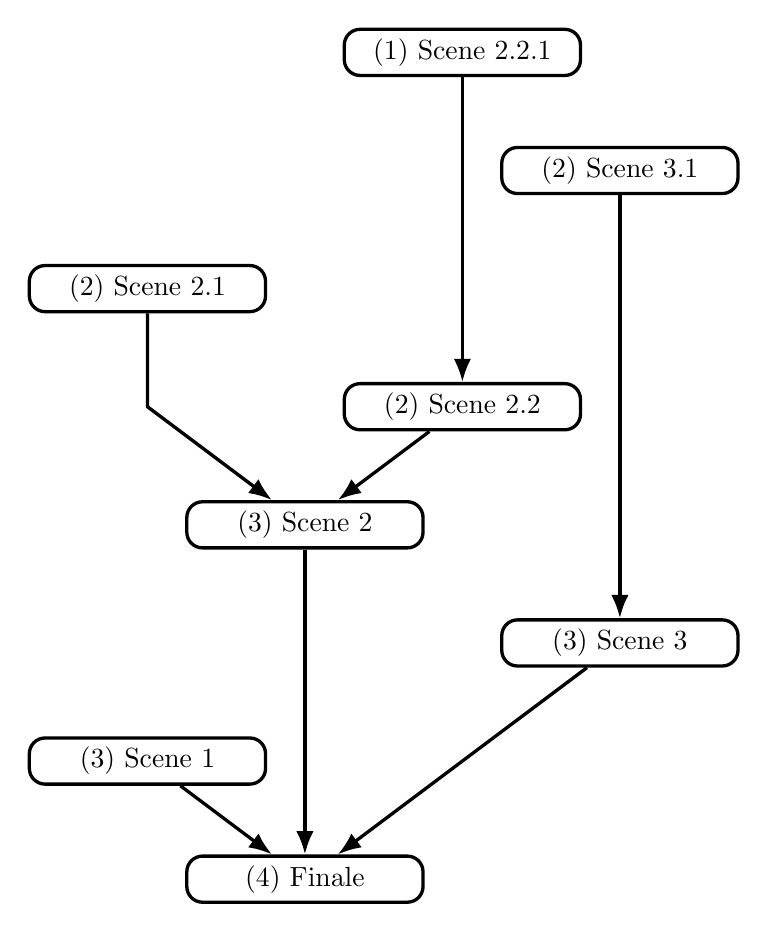
\begin{tikzpicture}[every path/.style={very thick}, every node/.style={draw, rounded corners=2mm, minimum width=3cm}]
\node (s1) at (0,0) {(4) Finale};
\node (s11) at (-2,1.5) {(3) Scene 1};
\node (s12) at (0,4.5) {(3) Scene 2};
\node (s13) at (4,3) {(3) Scene 3};
\node (s121) at (-2,7.5) {(2) Scene 2.1};
\node (s122) at (2,6) {(2) Scene 2.2};
\node (s131) at (4,9) {(2) Scene 3.1};
\node (s1221) at (2,10.5) {(1) Scene 2.2.1};

\draw[very thick, -{Latex}] (s11) -- (s1);
\draw[very thick, -{Latex}] (s12) -- (s1);
\draw[very thick, -{Latex}] (s13) -- (s1);
\draw[very thick,-{Latex}] (s121) -- (-2, 6) -- (s12);
\draw[very thick,-{Latex}] (s122) -- (s12);
\draw[very thick,-{Latex}] (s131) -- (s13);
\draw[very thick,-{Latex}] (s1221) -- (s122);
\end{tikzpicture}
\end{center}

The numbers in parentheses indicate the Difficulty Rating of the corresponding Scenes. This diagram implies an order in which the players might perform these Scenes, starting from the top with Scene 2.2.1 and progressing downwards to the Finale.

\newpage

\subsection*{Tell the Story}
During this phase, the players will tell the story of their Characters' adventures as they try to enact their plan to deal with the Catastrophe.
While the overall structure of the story is established when the players Write an Outline, when they Perform Scenes the players discover how the story unfolds and how the Characters are affected.

To Tell the Story, the players will Perform the Scenes described in the Outline.
A Scene cannot be Performed until after all of its Precursors have been Performed. Other than this restriction, however, the Scenes can be Performed in any order.

Before they make a Check to determine the Outcome of a Scene, the players should roleplay interactions between the Characters and the Objects that populate the Scene.
This is the players' opportunity to add new Objects to the Scene and Attach new Aspects to existing Objects.

After the Outcome of a Scene has been determined, the players should describe the Characters' actions in the Scene, how they led to the specified Outcome, and the narrative consequences of their actions.
This description should be informed by the pairs of Matching Aspects that the Characters attempted to use to manipulate the Scene to their advantage.
If the Scene was resolved successfully, then the players should describe which pairs of Matching Aspects they were able to exploit.
Otherwise, the players should describe what went wrong.

\newpage

\section*{The Moderator}
Optionally, one of the players can assume the role of \emph{Moderator}. The Moderator's job is to help the other players play the game. This assistance can take a variety of forms: from answering questions about the rules, managing logistics,  to ensuring that everyone agrees about various details of the story.

The Moderator should encourage the other players to tell an interesting story by asking them questions.  If the Moderator is curious about something in the story and wants to learn more,  then they should ask for more information.  Similarly, if the Moderator is confused then they should ask for clarification.

Importantly, however, the Moderator's role is not prescriptive.  The Moderator should not narrate any part of the story. The Moderator can make suggestions or present alternatives, but ultimately the other players should decide what happens.

\newpage

\section*{Modules}
The first thing that the players do in the game is Receive a Prophecy.  
This is the inciting incident for everything that happens in the story.
It's important!
By describing the prophesied Catastrophe, the players establish the foundation on which the rest the game will be built.

A \emph{Module} is a pre-written Prophecy designed  to help the players get started.
Each Module describes a Catastrophe as it might be presented to Characters who are hearing the Prophecy for the first time.  The players should read the Module aloud when they Receive the Prophecy and create Objects and Aspects to populate the fictional world that it implies.

\subsection*{Return of the Dragon}
Long ago, in the first age of men, the world was filled with wonders. 
The people of that time thought themselves safe from the fury of the natural world.
Then She came.
The great Dragon emerged from the sea and laid waste to the land.
Only the grandest works of those once great civilizations remain to mark their passage.

Or so the story goes.
Most scholars believe that the Dragon is a myth and that the Ancients were somehow responsible for their own demise.
Others believe that while the Dragon was real, She must surely have died long ago.
They are mistaken. 

After one thousand years of slumber, the Dragon wakes. 
The earth shakes as She begins to stir.
The oceans froth and swell as She shakes off the last vestiges of sleep.
Now we face the same fate as that which befell our forebears.

\newpage

\subsection*{Deep Impact}
My fellow Americans, it is with a heavy heart that I come to you tonight. 
As you are doubtless aware, last year the initial survey conducted as a part of Project Spaceguard discovered a large Near Earth Object that was projected to collide with the Earth later this month.
Ever since, the primary focus of this administration has been to prevent that from occurring. Earlier this evening, the director of Project Spaceguard informed me that we have failed.

Now, we must shift our focus from preventing a collision to surviving its aftermath.
Effective immediately, I am declaring a nationwide state of emergency.  National Guard units will be activated and deployed in support of local law enforcement. 

Going forward, the Federal Emergency Management Agency will be leading our response.
I'll turn the microphone over to the director of that agency now and he can provide details about what you can expect.
Goodnight and Godspeed.


\subsection*{She's Having a Baby}
Congratulations! It looks like you're at about eight weeks now.
Everything looks great, both mum and baby are doing fine. 
So, We'll plan on seeing you again in about four weeks.

While you're here I should tell you about the course that the hospital offers for new mums.
It's a great way to learn about what to expect and a chance talk to other new parents about the whole experience. 
The teachers are all former maternity ward nurses and they really do a great job.

I know that this can be overwhelming. If you have any concerns, please give us a call at any time.  OK?

\newpage

\section*{Acknowledgements}
Thanks to everyone who helped refine the design of Prophecy:
\begin{multicols}{2}
\begin{itemize}
  \item Keydan Bruce
  \item Farzana Choudhury
  \item Michael Cromer
  \item Dannielle Harden
  \item Andrew Hellyer
  \item Sarah Hewat
  \item Scott Joblin
  \item David McKenzie
  \item Paul Murray
  \item Kira Purcell
  \item Luke Purcell
  \item Jo Stephenson
  \item Brett Witty
  \item Bevis Worchester
  
\end{itemize}
\end{multicols}
\end{document}
